\documentclass[border=10pt]{standalone}

\usepackage{tikz}
\usepackage{tikzsymbols}
\usetikzlibrary{calc,patterns,shapes.geometric}

\def\centerarc[#1](#2)(#3:#4:#5){\draw[#1] ($(#2)+({#5*cos(#3)},{#5*sin(#3)})$) arc (#3:#4:#5);}

\begin{document}
	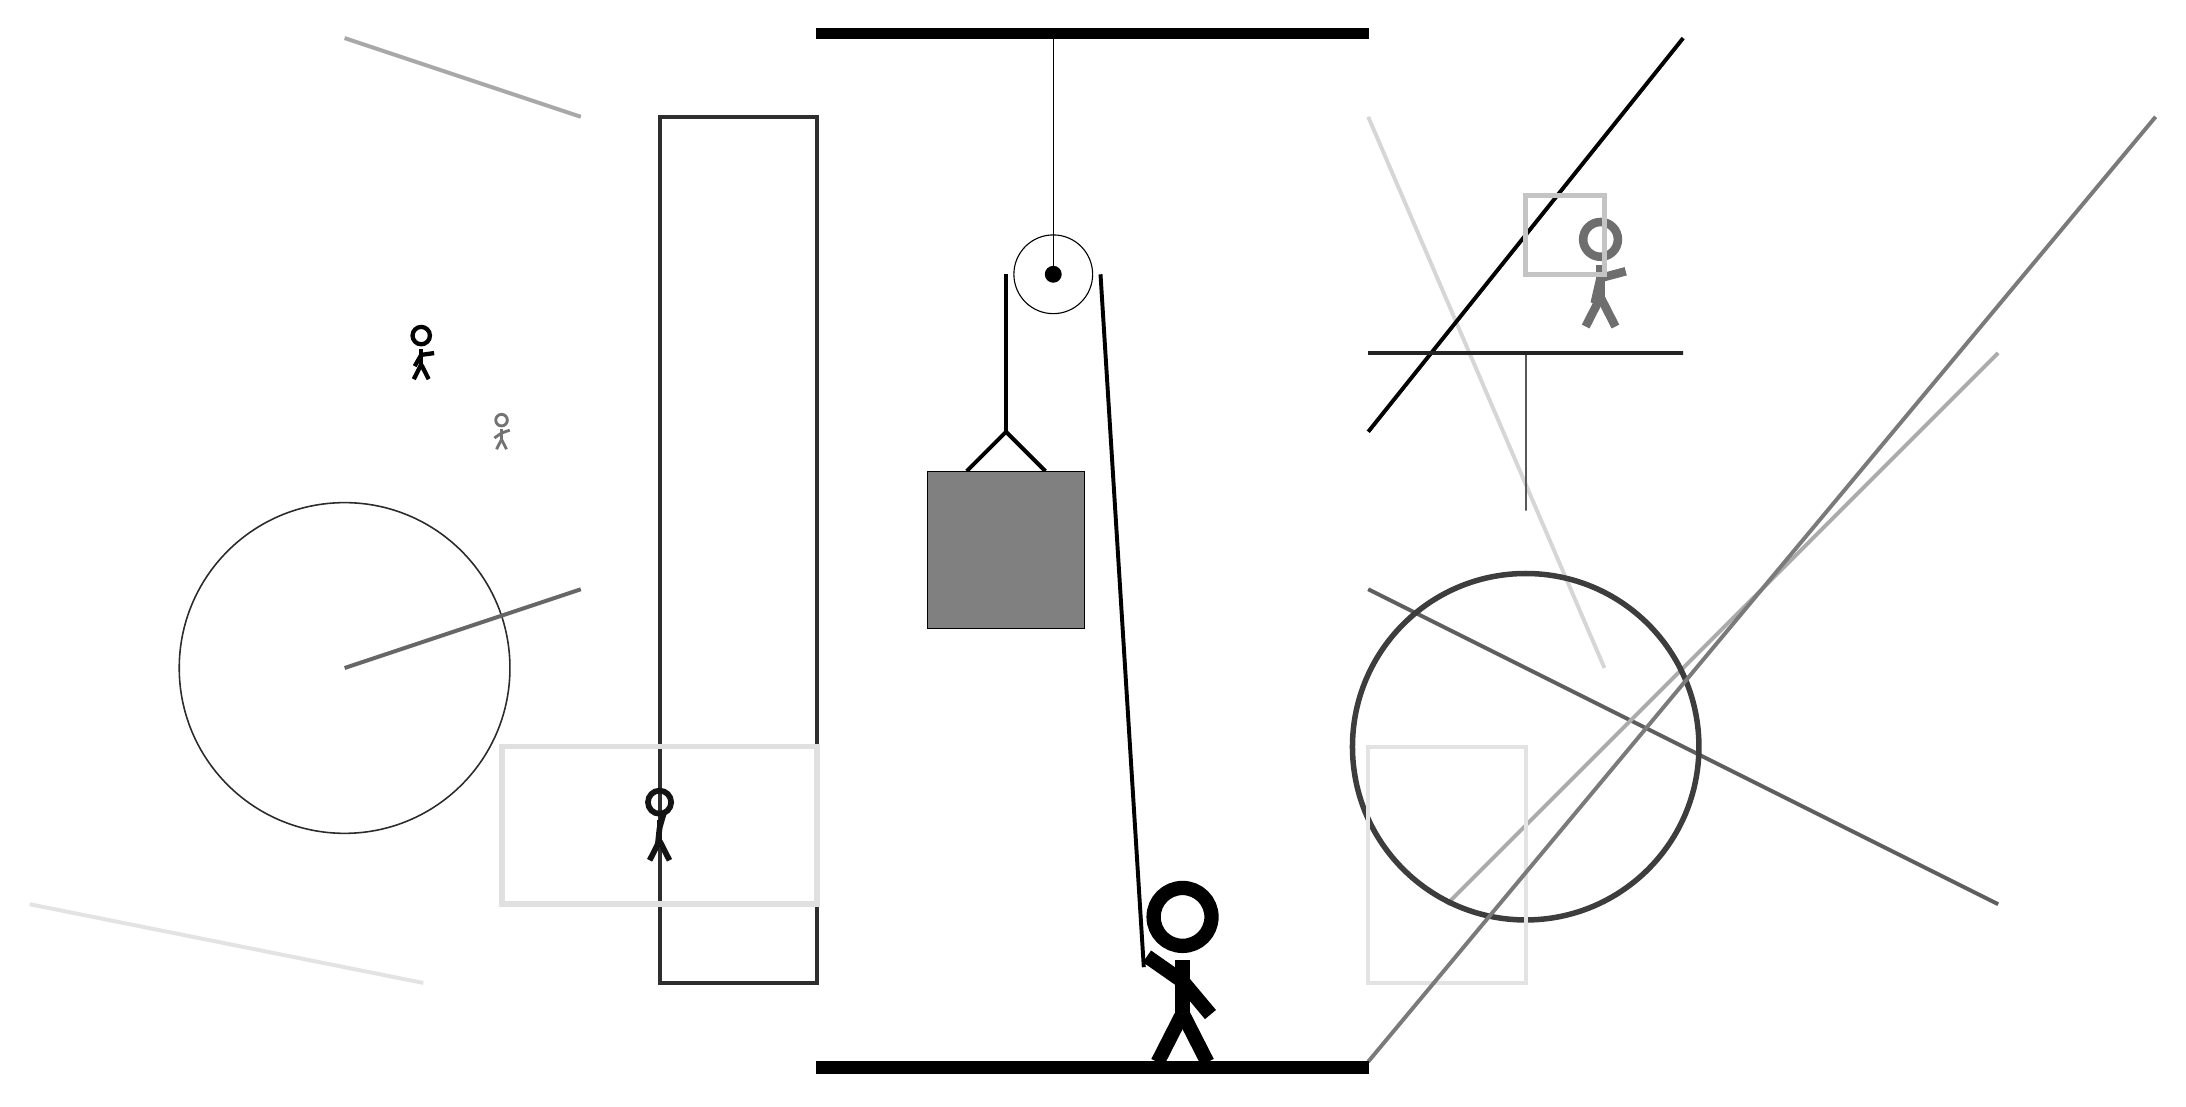
\begin{tikzpicture}
		%%%%% START %%%%%
		
		\draw[fill=black] (-2, 10) rectangle (5, 10.125);
		
		\draw (1, 7) circle (0.5);
		\draw[fill=black] (1, 7) circle (0.1);
		\draw (1, 10) -- (1, 7);
		
		\draw[line width=0.5mm] (-0.1, 4.5) -- (0.4, 5.0) -- (0.9, 4.5);
		\draw[fill=black!50] (-0.6, 4.5) rectangle (1.4, 2.5);
		
		\draw[line width=0.5mm, color=black!63](5, 3) -- (13, -1);
		
		\draw[line width=0.5mm, color=black!16](5, 9) -- (8, 2);
		\draw[line width=0.5mm, color=black!33](6, -1) -- (13, 6);
		\draw[line width=0.5mm, color=black!82] (-2, 9) rectangle (-4, -2);
		
		\draw [line width=0.2mm, color=black!83](-8, 2) circle (2.1);
		\draw [line width=0.7mm, color=black!76](7, 1) circle (2.2);
		\node[line width=0.3mm, color=black!55] at (-6, 5) {\Strichmaxerl[2][35][19]};
		\draw[line width=0.5mm, color=black!99](5, 5) -- (9, 10);
		\draw[line width=0.5mm, color=black!60](-5, 3) -- (-8, 2);
		\draw[line width=0.2mm, color=black!66] (7, 6) rectangle (7, 4);
		\draw[line width=0.5mm, color=black!86] (5, 6) rectangle (9, 6);
		
		\draw[line width=0.7mm, color=black!12] (-2, -1) rectangle (-6, 1);
		\draw[line width=0.5mm, color=black!11] (7, 1) rectangle (5, -2);
		\node[line width=0.2mm, color=black!57] at (8, 7) {\Strichmaxerl[6][77][15]};
		\node[line width=0.6mm, color=black!99] at (-7, 6) {\Strichmaxerl[3][60][8]};
		\draw[line width=0.5mm, color=black!52](5, -3) -- (15, 9);
		
		\draw[line width=0.6mm, color=black!23] (7, 7) rectangle (8, 8);
		\node[line width=0.7mm, color=black!92] at (-4, 0) {\Strichmaxerl[4][84][74]};
		\draw[line width=0.5mm, color=black!11](-7, -2) -- (-12, -1);
		
		\draw[line width=0.5mm, color=black!34](-5, 9) -- (-8, 10);
		
		\draw[line width=0.5mm] (0.4, 7) -- (0.4, 5.0);
		\centerarc[line width=0.5mm](1, 7)(0:180:0.6);
		\draw[line width=0.5mm](1.6, 7) -- (2.15, -1.8);
		
		\node at (2.6, -1.9) {\Strichmaxerl[10][-35][-50]};
		
		\draw[fill=black] (-2, -3) rectangle (5, -3.15);
		
		%%%%% END %%%%%
	\end{tikzpicture}
\end{document}